\ylDisplay{Kiirtekimbu laiendi} % Ülesande nimi
{Tundmatu autor} % Autor
{piirkonnavoor} % Voor
{2010} % Aasta
{G 3} % Ülesande nr.
{2} % Raskustase
{
% Teema: Geomeetriline-optika
\ifStatement
Kaks ühise optilise peateljega läätse moodustavad seadme, millega saab paralleelsest valgusvihust moodustada esialgsest laiema või kitsama paralleelse valgusvihu. Kasutatava seadme esimese läätse optiline tugevus on \SI{-20}{dpt}. Kui kaugele esimesest läätsest tuleks paigutada teine lääts, et laiendada seadmele langev valgusvihk \num{2.5}-kordseks?
\fi


\ifHint
Selleks, et sisenev kiirte kimp oleks ka peale teise läätse läbimist paralleelne, peavad läätsede fookused ühtima.
\fi


\ifSolution
\begin{center}
	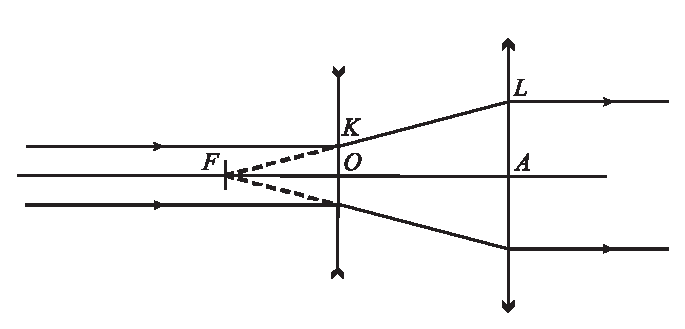
\includegraphics[width=0.7\textwidth]{2010-v2g-03-laiendi.eps}
\end{center}

Kuna esimese läätse optiline tugevus on negatiivne, on see nõgus. Selleks, et sisenev paralleelne valgusvihk püsiks paralleelne peale süsteemist väljumist, peavad läätsede fookused ühtima. Olgu vastav ühine fookus $F$. Lisaks olgu läätsede keskpunktid $O$ ja $A$ ning siseneva kiirtekimbu kõige äärmise kiire lõikepunktid läbi läätsede $K$ ja $L$.

Sellisel juhul saame kolmnurkade $KOF$ ja $LAF$ sarnasusest, et 
\[
\frac{|LA|}{|KO|}=\frac{|AF|}{|OF|}.
\]
Kuna $|AL| = \num{2.5}|OK|$, siis $|AF| = \num{2.5}|OF|$, ehk läätsede vahekaugus on 
\[
|OA| = |AF| - |OF| = \num{1.5}|OF| = \num{1.5} \left\lvert\frac{\SI{1}{m}}{\num{-20}}\right\rvert = \SI{7.5}{cm}.
\]
\fi
}